\chapter{RESULTS AND DISCUSSIONS}
\thispagestyle{empty}
\onehalfspacing
\pagestyle{fancy}
\fancyhf{}
\fancyhead[LE,RO]{\textit{\footnotesize \thepage}}
\fancyhead[RE,LO]{\textit{\footnotesize WHALING-GUARD : PHISHING DETECTION USING MACHINE LEARNING}}
%\fancyfoot[LE,LO]{\textit{\footnotesize Department of CSE}}
\fancyfoot[LE,RO]{\textit{\footnotesize Department of CSE}}
 
\renewcommand{\headrulewidth}{2pt}
\renewcommand{\footrulewidth}{1pt}


\section{Feature Analysis}
\subsection*{Boxplot Graph}
\par The boxplot graph is a useful visualization for displaying the distribution of a numerical feature or variable. It is employed to explore and understand the distribution of feature values during the analysis of the dataset.By creating the boxplot graph, we could gain insights into the distribution of feature values, including measures of central tendency, dispersion, mean and identification of outliers. Visualization of some features are shown below:

\begin{figure}[H]
  \centering
  \subfloat[getEntropy]{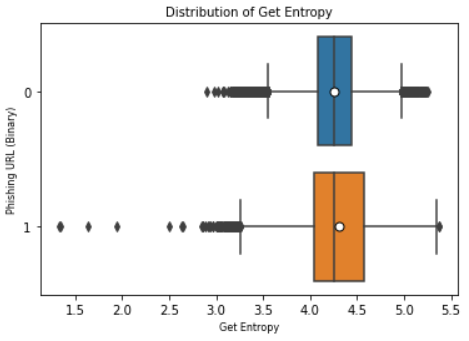
\includegraphics[width=0.45\textwidth]{getEntropy.png}\label{fig:figure1}}
  \hfill
  \subfloat[hasLogin]{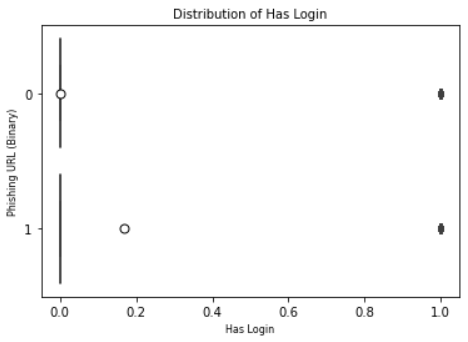
\includegraphics[width=0.450\textwidth]{hasLogin.png}\label{fig:figure2}}
  \label{fig:bothfigures}
\end{figure}

\begin{figure}[H]
  \centering
  \subfloat[getDepth]{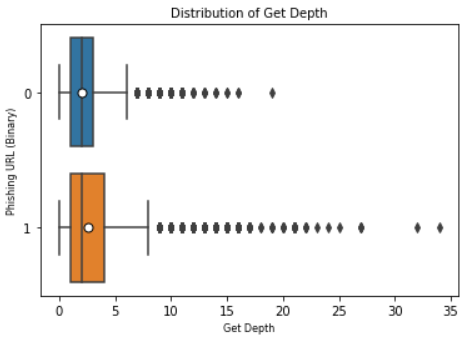
\includegraphics[width=0.450\textwidth]{getDepth.png}\label{fig:figure1}}
  \hfill
  \subfloat[urlLength]{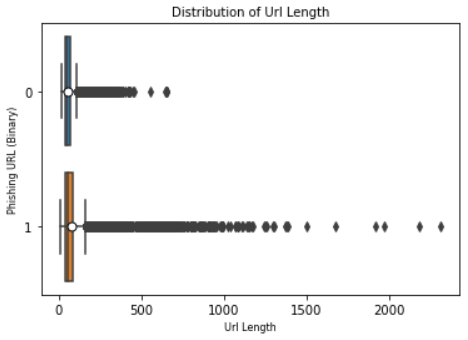
\includegraphics[width=0.450\textwidth]{urlLength.png}\label{fig:figure2}}
  \caption{Visualization of URL features}
  \label{fig:bothfigures}
\end{figure}

\par Visually, we see that legitimate URLs have higher entropy and are generally longer than phishing URLs.Similarly, we can capture the fact that ‘red flag’ keywords appear in a URL string which is the keyword ‘login’, is more seen in the phishing URLs. The depth of the url i.e, number of hierarchical levels or directories in the URL’s path for phishing URLs is seen greater than the legitimate ones. It is also seen that the phishing URLs have higher url length than the legitimate URLs.

\section{Pycaret Checking}

\begin{figure}[H]
\centerline{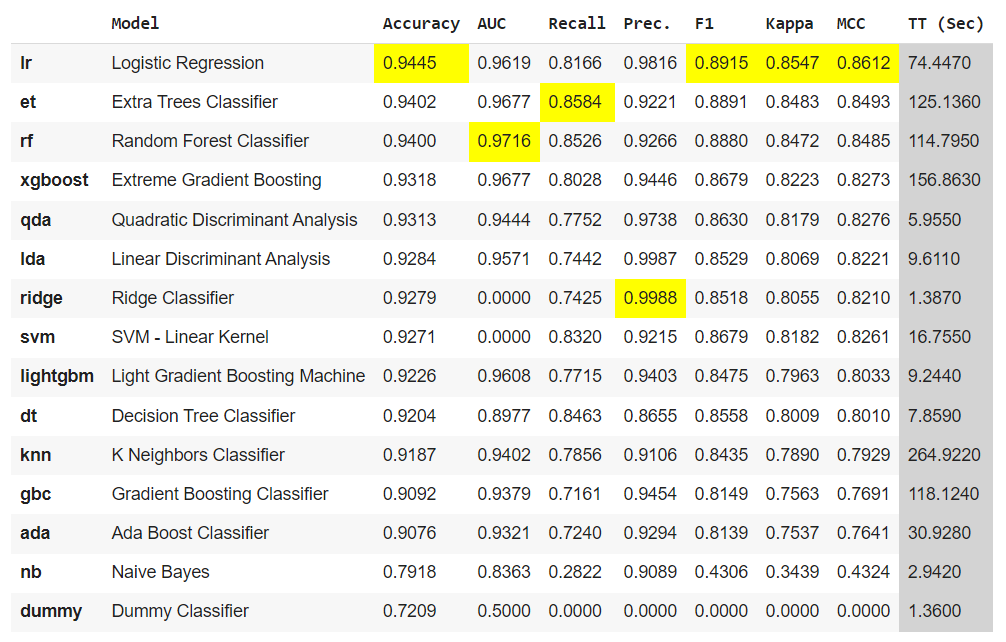
\includegraphics[scale=0.6]{pycaretCheck.png}}
\caption{Pycaret Comparison}
\label{fig}
\end{figure}

\par When using PyCaret for model comparison, the results obtained can provide valuable insights into the performance of different machine learning algorithms on the given dataset.The comparison results obtained using PyCaret can guide in selecting the most suitable machine learning model(s) for this project, taking into account performance metrics, statistical significance, feature importance, and other relevant factors. Fig:5.3 shows the comparison result.
\section{Model Analysis}
\begin{figure}[H]
\centerline{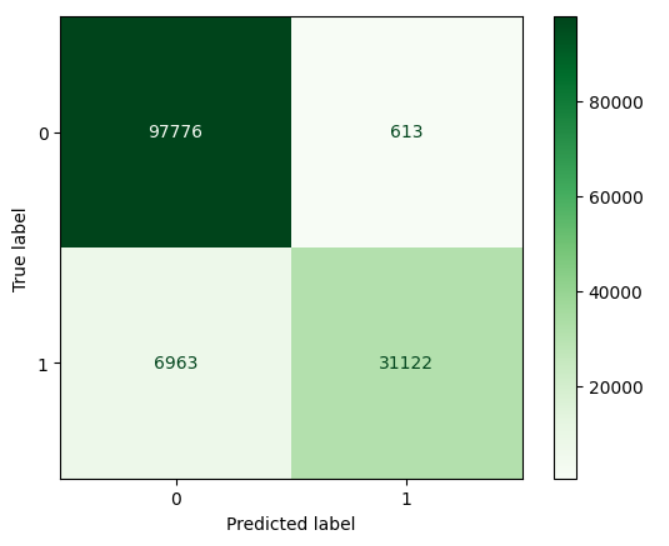
\includegraphics[scale=0.6]{greenCN.png}}
\caption{Confusion Matrix}
\label{fig}
\end{figure}


\par A confusion matrix is a table that is used to evaluate the performance of a classification model. It shows the number of true positives (TP), true negatives (TN), false positives (FP), and false negatives (FN) by comparing the predicted labels with the true labels of a dataset. The confusion matrix provides a more detailed understanding of the model's performance beyond simple accuracy. From the confusion matrix, some of the evaluation metrics calculated in our project are shown in fig:5.5
\begin{figure}[H]
\centerline{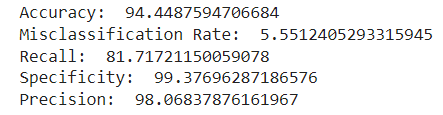
\includegraphics[scale=0.8]{CMvalues.png}}
\caption{Evaluation metrics}
\label{fig}
\end{figure}
\par Based on the Logistic Regression Model, it has assigned feature importance score to each extracted features. It helps to provide insights into which features have the most influence on the model's predictions. Fig:5.6 shows the importance of some of the features in our project in the descending order.
\begin{figure}[H]
\centerline{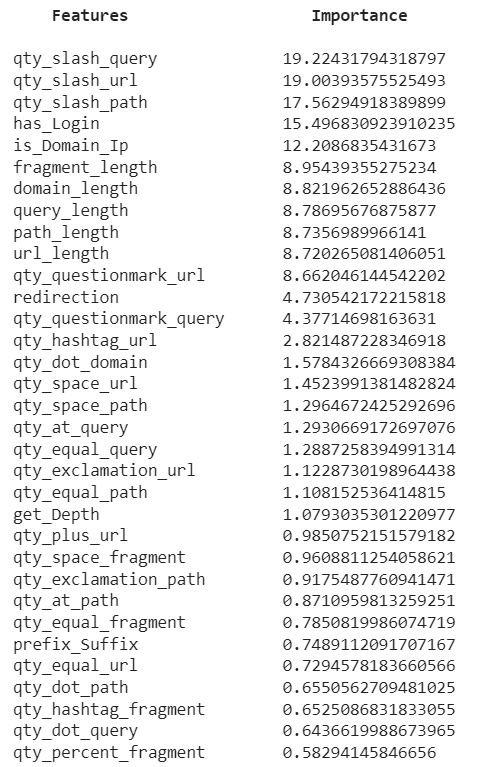
\includegraphics[scale=0.8]{featImp1.png}}
\caption{Features and their importances}
\label{fig}
\end{figure}

\section{Web Application}
\par We have developed a web application where the users can input urls to check if it is phishing or non-phishing.The UI of the application is developed using Reactjs and the API setup for the application is implemented using Nodejs. Fig:5.7 shows the User Interface of the WhalingGuard web application.
\begin{figure}[H]
\centerline{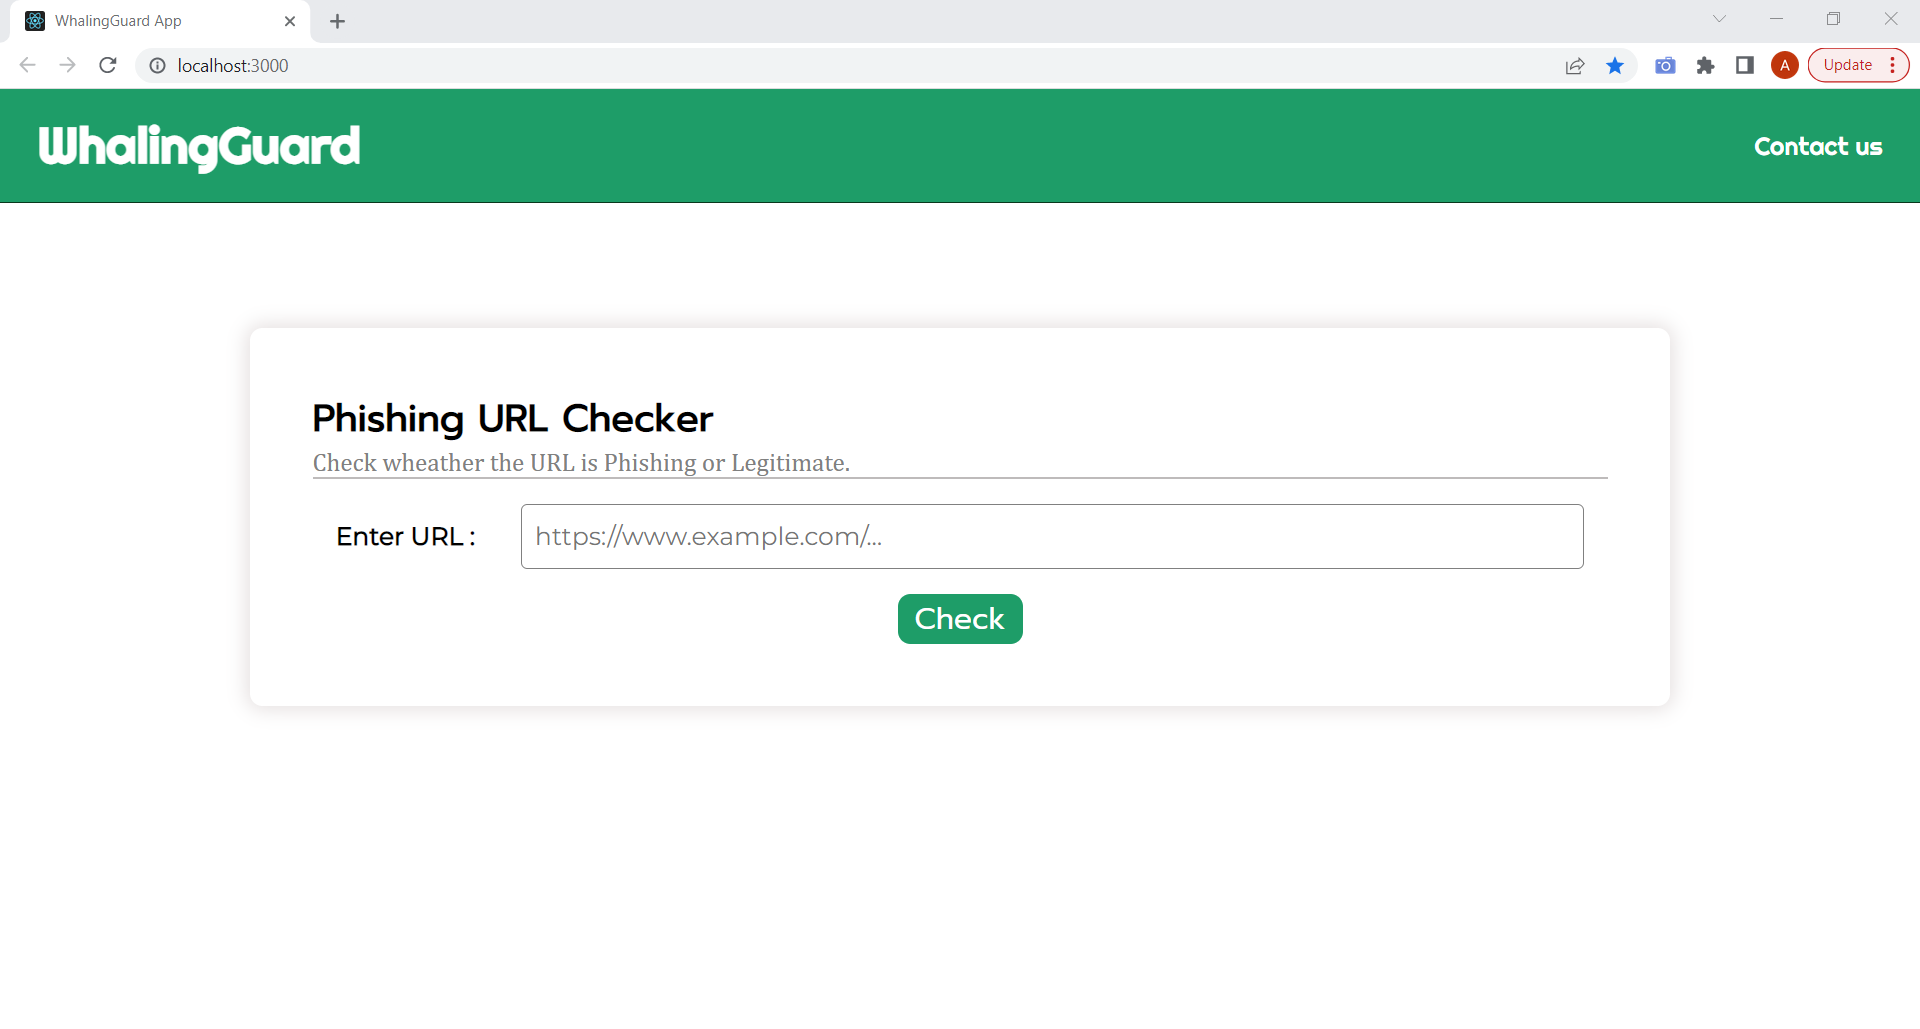
\includegraphics[scale=0.35]{ui.png}}
\caption{User Interface}
\label{fig}
\end{figure}
\par The URL entered by the user is received by the server and it is predicted by the evaluated LR model.Based on the prediction, the summary of the result is shown as output in the user-interface. The following figures shows the 2 different output produced.
\begin{figure}[H]
\centerline{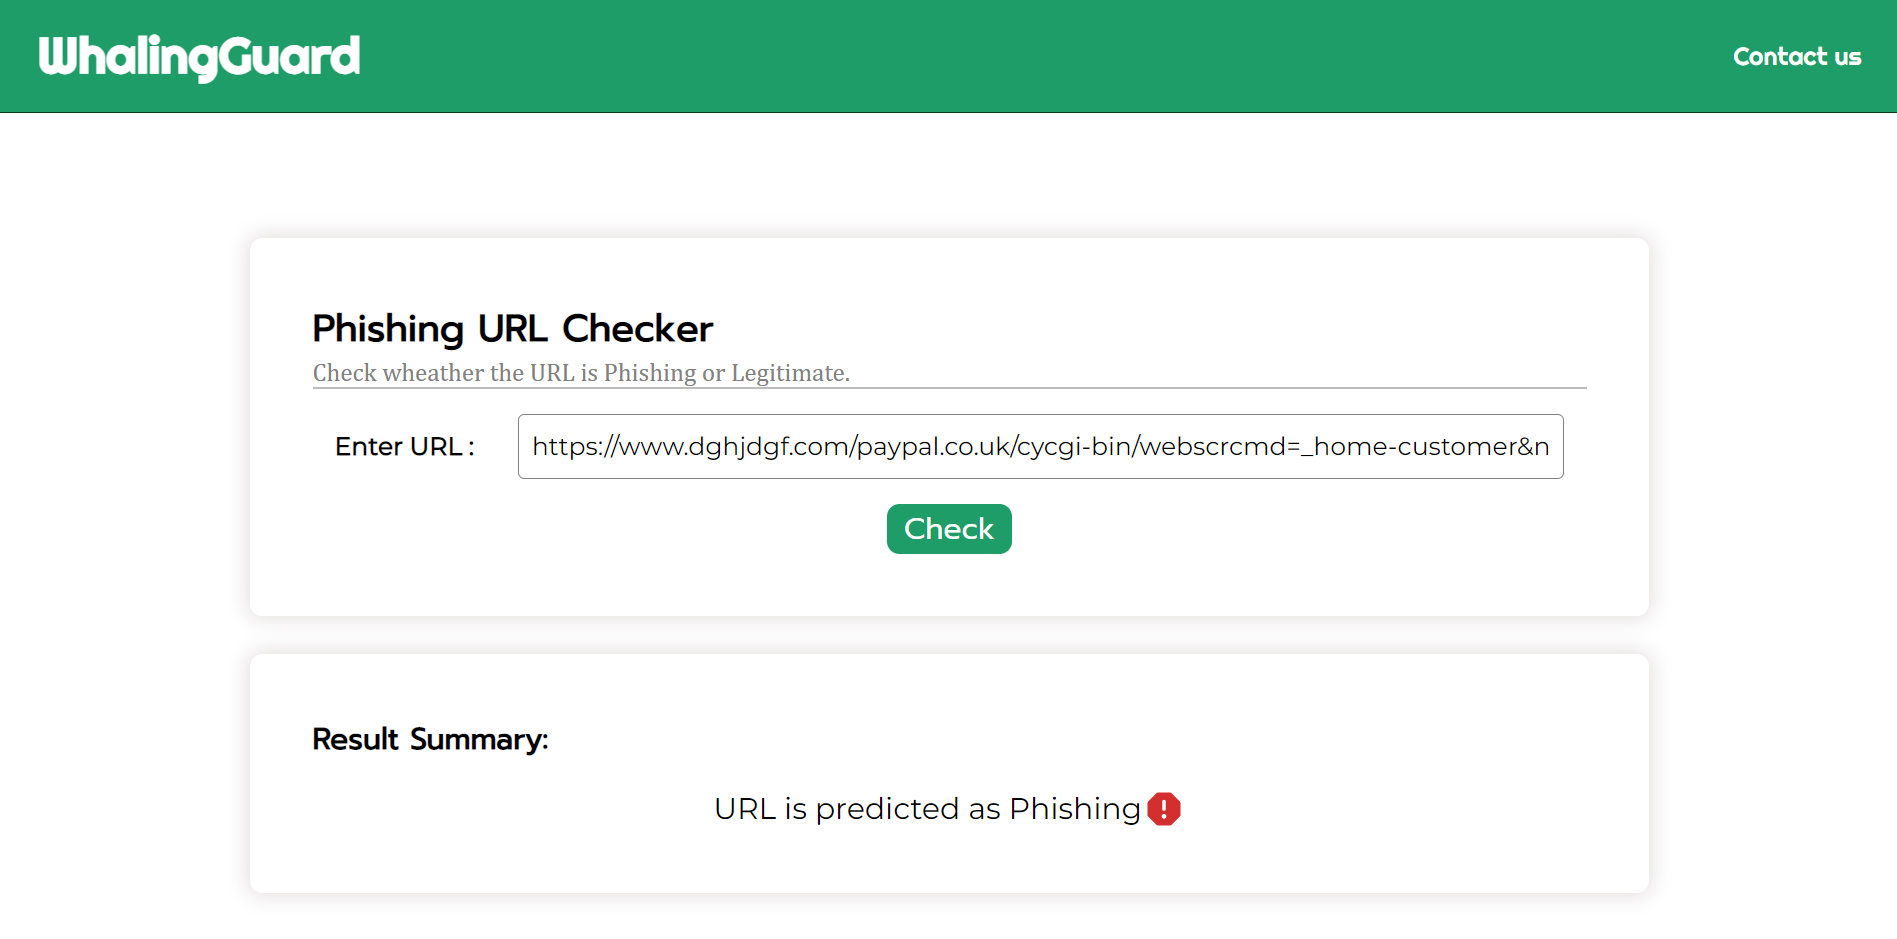
\includegraphics[scale=0.35]{uiP.png}}
\end{figure}
\begin{figure}[H]
\centerline{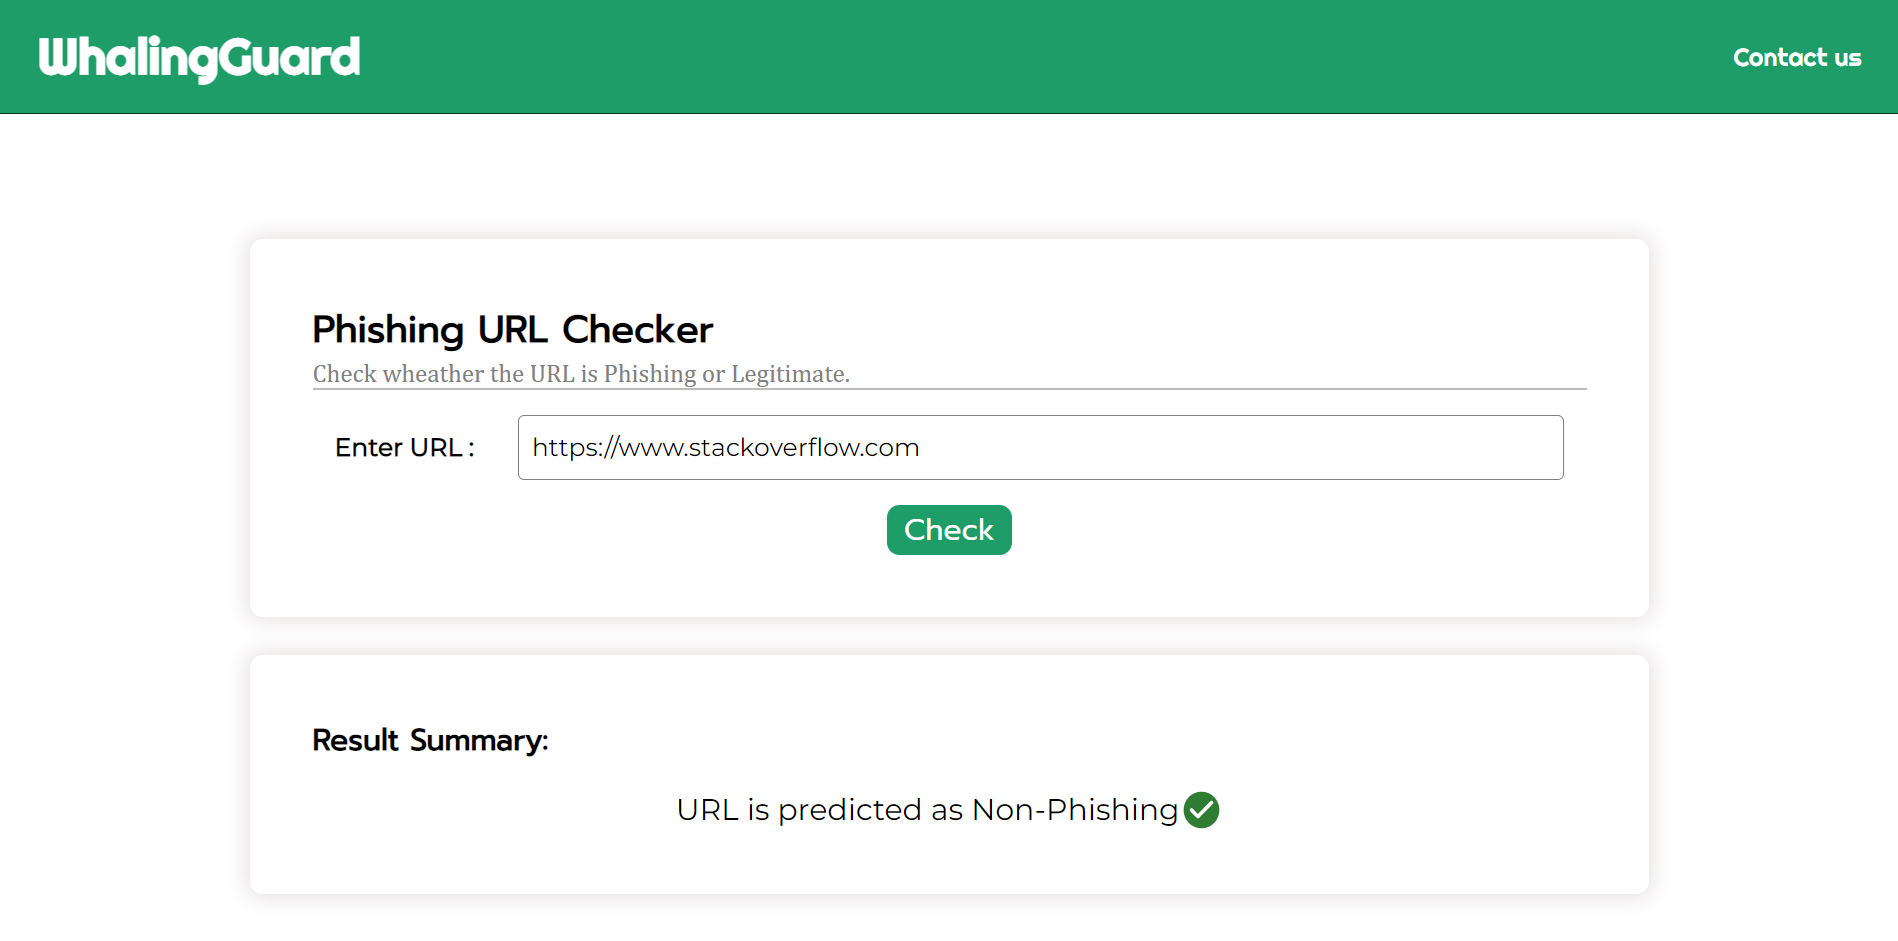
\includegraphics[scale=0.35]{uiN.png}}
\caption{Prediction Results}
\label{fig}
\end{figure}










